\section{Methodology}
\label{sec:method}

In this section, we first provide an overview of the proposed methodology, followed by a detailed introduction of its components.

\begin{figure*}[t]
  \centering
  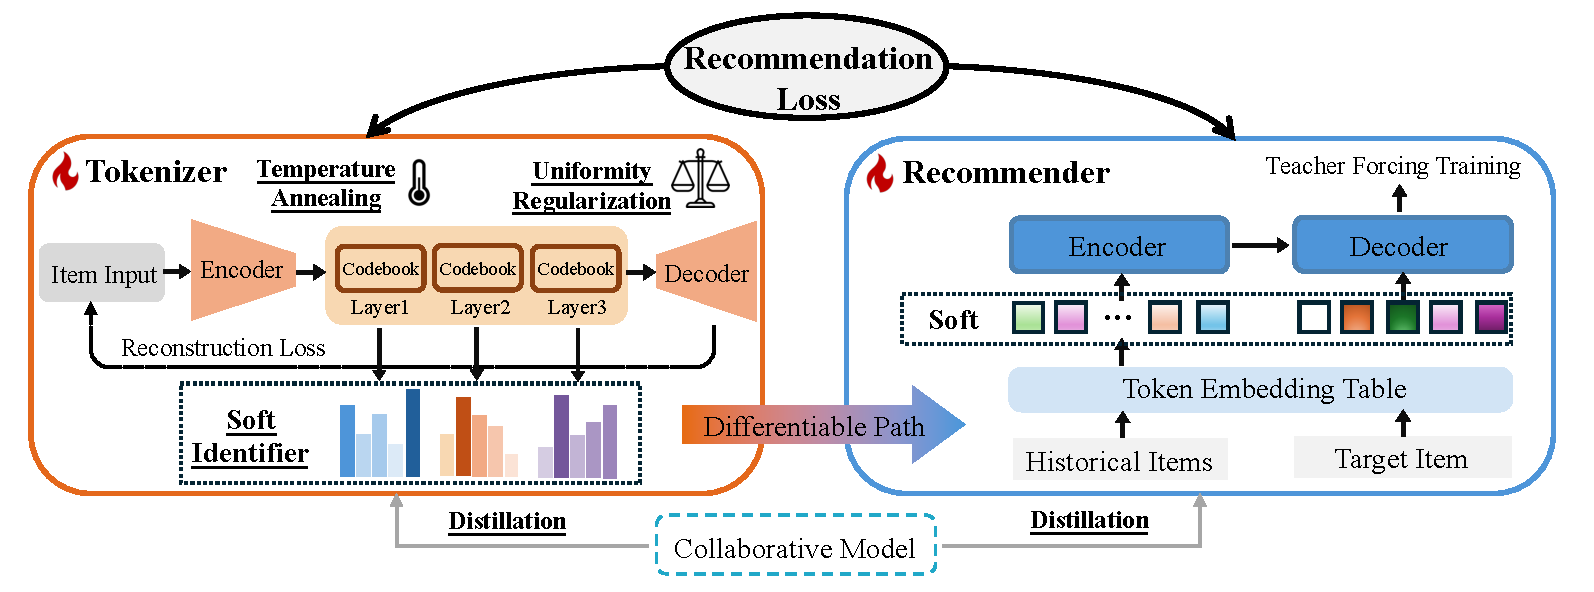
\includegraphics[width=0.95\textwidth]{figure/framework.pdf}
    \caption{Overview of the proposed UniGRec framework. By introducing soft identifiers, the tokenizer and recommender are seamlessly integrated, enabling end-to-end joint optimization under a unified recommendation objective. Temperature annealing and uniformity regularization are crucial for practical effectiveness, while a pre-trained lightweight teacher model offers additional collaborative supervision.}

  \label{fig:framework}
\end{figure*}

\subsection{Overview}
We aim to unify the tokenizer and the recommender under a single objective and perform end-to-end joint optimization, rather than training them sequentially or optimizing them asynchronously. This design simplifies the training pipeline and leads to better alignment between the two components. Our key belief is that the ultimate recommendation loss can serve as a unified objective for both modules. To overcome the non-differentiability of hard identifiers, we adopt the \textit{soft identifier}, which replace discrete codewords with continuous assignment probabilities.

Based on this idea, we introduce \textbf{UniGRec} (Unified Generative Recommendation), a unified framework for jointly optimizing the tokenizer and the recommender (Figure~\ref{fig:framework}). UniGRec comprises three components: (1) \textit{Annealed Inference Alignment}, which mitigates the training–inference mismatch induced by soft-to-hard identifier transitions; (2) \textit{Codeword Uniformity Regularization}, which alleviates item identifier collapse caused by over-concentration on dominant codewords; and (3) \textit{Dual Collaborative Distillation}, which compensates for insufficient collaborative supervision by transferring collaborative priors from a lightweight teacher model.


\subsection{Annealed Inference Alignment}
We first introduce the formulation of soft identifiers, and then present the annealing strategy applied to the assignment logits to align training and inference process.

\subsubsection{Soft Identifiers}
Our approach builds upon RQ-VAE~\cite{TIGER}. As shown in Equation~\eqref{eq:assgin}, RQ-VAE assigns each item to its nearest codeword at each quantization layer, resulting in a one-hot identifier. While effective, such hard identifiers exhibit two inherent limitations. First, they incur information loss, as an item may be semantically close to multiple codewords but is forced to select only the nearest one. Second, hard assignments impede joint optimization: the $\arg\min$ operation is non-differentiable, preventing gradients from propagating from the recommendation objective back to the tokenizer. Consequently, although the recommender operates on tokenized representations, the two modules cannot be effectively aligned under a unified training objective.

To address these issues, we adopt \textit{soft identifiers}. Instead of selecting a single codeword, we represent each item as a probability distribution over all codewords. Specifically, we treat the negative squared distances between the residual representation $\bm{r}_{l-1}$ and the codewords $\{\bm{e}_l^k\}_{k=1}^{K}$ as logits, apply temperature scaling, and compute assignment probabilities via a softmax function:
\begin{equation}\label{eq:soft_prob}
p_l(k) = \frac{\exp \left( - \| \bm{r}_{l-1} - \bm{e}_l^k \|^2 / \tau \right)}{\sum_{j=1}^{K} \exp \left( - \| \bm{r}_{l-1} - \bm{e}_l^j \|^2 / \tau \right)}, \quad k=1,\cdots, K, 
\end{equation}
where $\tau$ denotes the temperature parameter controlling the sharpness of the assignment distribution. 

Consequently, the discrete code selection is replaced by a probability-weighted aggregation of codewords. These soft assignments preserve richer semantic information and, more importantly, enable fully differentiable end-to-end optimization, allowing the recommendation objective to directly supervise the tokenizer.

To feed soft identifiers into the recommender, we further adapt the input representation. Note that the assignment distribution $p_l(\cdot)$ is defined over $K$ codewords, which is typically much smaller than the full token vocabulary size $|\mathcal{V}|$ of the recommender. Therefore, we first initialize a zero vector with the same dimensionality as the token vocabulary, and then scatter the assignment probabilities corresponding to the codewords of the current quantization layer into their respective token positions. Concretely, we replace the standard embedding lookup with a probability-weighted embedding aggregation. 
Taking the encoder input token $\bm{o}_l^t$ in Equation~\eqref{eq:rec_input} as an example, we compute it as:
\begin{equation}\label{eq:new_rec_input}
\bm{o}_l^t = \text{scatter}\big(\bm{0}, \{p_l(k)\}_{k=1}^{K}\big)\cdot \bm{\mathcal{O}},
\end{equation}
where $\text{scatter}(\cdot)$ maps the $K$-dimensional assignment probabilities to their corresponding indices in the full vocabulary space, producing a sparse $|\mathcal{V}|$-dimensional vector, and $\bm{\mathcal{O}} \in \mathbb{R}^{|\mathcal{V}| \times D}$ denotes the token embedding table of the recommender. This formulation reduces to standard embedding lookup when $p_l(\cdot)$ degenerates to a one-hot vector, while remaining fully differentiable with respect to the tokenizer parameters.


\subsubsection{Temperature Annealing}
Although the proposed design enables end-to-end optimization between the tokenizer and the recommender, it introduces a \textit{Training–Inference Discrepancy}: the recommender is trained with soft identifiers, whereas inference requires deterministic item representations. To mitigate this issue, we apply a linear annealing strategy to the temperature parameter $\tau$ in Equation~\eqref{eq:soft_prob}, progressively reducing it during training:
\begin{equation}\label{eq:tau_sche}
    \tau(\text{step}) = \tau_{\max} - \frac{\text{step}}{\text{total\_step}} \left(\tau_{\max} - \tau_{\min}\right),
\end{equation}
where $\text{step} \in [0, \text{total\_step}]$ denotes the current training step, and $\tau_{\max}$ and $\tau_{\min}$ are the initial (maximum) and final (minimum) temperatures, respectively.

As $\tau$ decreases, the soft assignment distribution becomes increasingly peaked, concentrating probability mass on the nearest codeword. Consequently, the soft weighted embedding gradually converges to the deterministic embedding obtained via hard assignment. This annealed inference alignment enables smooth, fully differentiable optimization in early training, while progressively matching the inference-time behavior.

\subsection{Codeword Uniformity Regularization}

As shown in Equation~\eqref{eq:soft_prob}, each item interacts with the full codebook at the gradient level, which can bias optimization toward a few dominant codewords. In our experiments, this often leads to severe codeword usage imbalance, a phenomenon we term \emph{Item Identifier Collapse}, consistent with prior work~\cite{EdVAE,Zhu_2025_ICCV}. 

To address this, we regularize the codeword assignment probabilities to promote uniform usage, computing batch-level averages to reduce noise and stabilize training. Specifically, we introduce a diversity loss to penalize low-entropy distributions:
\begin{equation}\label{eq:CU}
    \mathcal{L}_\text{CU} = \sum_{l=1}^{L} \sum_{k=1}^{K} \bar{p}_l(k) \log (\bar{p}_l(k)),
\end{equation}
where $\bar{p}_l(k)$ denotes the batch-averaged assignment probability of the $k$-th codeword at the $l$-th quantization level. Minimizing $\mathcal{L}_\text{CU}$ is equivalent to minimizing the KL divergence between $\bar{p}_l$ and a uniform distribution, thereby encouraging more balanced codeword utilization.

\subsection{Dual Collaborative Distillation}

Although soft identifiers are effective at modeling fine-grained, token-level semantics, this emphasis may partially weaken the modeling of coarse-grained, item-level collaborative signals, which provide complementary supervision that is not fully captured by tokenized representations alone~\cite{LETTER,DiscRec}. 

To mitigate this limitation, we introduce a pretrained ID-based collaborative recommender (SASRec~\cite{SASRec}) as a teacher model and leverage its item ID embeddings to supplement collaborative knowledge.
Specifically, we perform collaborative distillation from two complementary perspectives, as detailed below:


\subsubsection{Tokenizer Side}

Our goal on the tokenizer side is to inject collaborative priors into the codebook space, encouraging the soft assignment distributions to align with the quantized representations derived from the collaborative teacher embeddings. To this end, we first extract the historical sequence representation from the recommender encoder, denoted as $\bm{h}^\text{Enc}$ (obtained via average pooling over $\bm{H}^\text{Enc}$ in Equation~\eqref{eq:rec_encoder}), and the unique target item embedding from the pretrained collaborative teacher model, denoted as $\bm{h}^\text{Tea}$. We then project these representations through a linear layer to match the input dimension of the tokenizer and feed them into the tokenizer to obtain the codebook assignment probability distributions, denoted as $P_l^\text{Enc}=\{p_l(k)^\text{Enc}\}_{k=1}^K$ and $P_l^\text{Tea}=\{p_l(k)^\text{Tea}\}_{k=1}^K$, respectively. The subscript $l$ indicates that these distributions correspond to the $l$-th quantization layer.


Finally, we define a symmetric KL divergence loss between the two distributions for each codeword:
\begin{equation}\label{eq:CDT}
    \mathcal{L}_\text{CD}^\mathcal{T} = \sum_{l=1}^{L} \left[ D_{KL}\big(P_l^\text{Enc} \,\|\, P_l^\text{Tea}\big) + D_{KL}\big(P_l^\text{Tea} \,\|\, P_l^\text{Enc}\big) \right],
\end{equation}
where $D_{KL}(\cdot \| \cdot)$ denotes the KL divergence. 



\subsubsection{Recommender Side}

On the recommender side, our goal is to inject collaborative priors directly into the item embedding space, encouraging the recommender to produce representations that are consistent with those of a pretrained collaborative teacher. Specifically, for a target item $i_{T+1}$, we extract its representation from the recommender decoder, denoted as $\bm{h}^\text{Dec}_i$ (obtained via first-token pooling from $\bm{H}^\text{Dec}$ in Equation~\eqref{eq:rec_decoder}), and the corresponding embedding from the pretrained teacher model, denoted as $\bm{h}^\text{Tea}_i$. We then project $\bm{h}^\text{Dec}_i$ through a linear layer to match the teacher embedding dimension and employ an in-batch InfoNCE loss to align the recommender outputs with the teacher embeddings.

Formally, for two sets of embeddings, $A = \{\bm{a}_i\}$ and $B = \{\bm{b}_i\}$, we define the InfoNCE loss as
\begin{equation}
\mathcal{L}_\text{InfoNCE}(A, B) 
= - \sum_{i} \log \frac{\exp(\text{sim}(\bm{a}_i, \bm{b}_i) / \tau')}
{\sum_{j} \exp(\text{sim}(\bm{a}_i, \bm{b}_j) / \tau')},
\end{equation}
where $\text{sim}(\cdot, \cdot)$ denotes the cosine similarity function and $\tau'$ is a temperature hyperparameter distinct from that used elsewhere.
To enforce bidirectional alignment, we define the recommender-side collaborative distillation loss as:
\begin{equation}\label{eq:CDR}
\mathcal{L}_\text{CD}^\mathcal{R} =
\mathcal{L}_\text{InfoNCE}(\{\bm{h}_i^\text{Dec}\}, \{\bm{h}_i^\text{Tea}\})
+ \mathcal{L}_\text{InfoNCE}(\{\bm{h}_i^\text{Tea}\}, \{\bm{h}_i^\text{Dec}\}),
\end{equation}
where the first term treats the recommender embeddings as queries and the teacher embeddings as keys, and the second term reverses the roles to achieve symmetric distillation.


\begin{algorithm}[t]
\caption{Training Pipeline of UniGRec}
\label{alg:training}
\begin{algorithmic}[1]

\State \textbf{Initialize:} Tokenizer $\mathcal{T}$, Recommender $\mathcal{R}$;

\State \textbf{// Stage 1: Tokenizer Pretraining}
\While{not converged}
    \State Sample a mini-batch of items;
    \State Update temperature $\tau$ via Equation~\eqref{eq:tau_sche};
    \State Compute assignment probabilities $p_l(k)$ via Equation~\eqref{eq:soft_prob};
    \State Compute reconstruction loss $\mathcal{L}_\text{Recon}$ 
    via Equation~\eqref{eq:rqvae_loss};
    \State Compute regularization term $\mathcal{L}_\text{CU}$ via Equation~\eqref{eq:CU};
    \State Update $\mathcal{T}$ by minimizing $\mathcal{L}_\text{Pre}$ in Equation~\eqref{eq:pre};
\EndWhile


\State \textbf{// Stage 2: End-to-End Joint Training}
\State Fix temperature $\tau \gets \tau_{\min}$;
\While{not converged}
    \State Sample a mini-batch of interactions;

    \State Compute reconstruction loss $\mathcal{L}_\text{Recon}$ 
    via Equation~\eqref{eq:rqvae_loss};

    \State Compute inputs of soft identifier via Equation~\eqref{eq:new_rec_input};

    \State Compute recommendation loss $\mathcal{L}_\text{Rec}$ via Equation~\eqref{eq:loss_rec};

    \State Compute tokenizer-side distillation $\mathcal{L}_\text{CD}^\mathcal{T}$ via Equation~\eqref{eq:CDT};
    
    \State Compute recommender-side distillation $\mathcal{L}_\text{CD}^\mathcal{R}$ Equation~~\eqref{eq:CDR};

    \State Update $\mathcal{T}, \mathcal{R}$ by minimizing $\mathcal{L}_\text{Joint}$ in Equation~\eqref{eq:joint};
\EndWhile

\end{algorithmic}
\end{algorithm}

\subsection{Training Pipeline}\label{sec:pipeline}

We summarize the overall training procedure of UniGRec in Algorithm~\ref{alg:training}, which proceeds in two progressive stages:

\subsubsection{Stage 1: Tokenizer Pretraining} 
In practice, the tokenizer generally requires substantially more epochs to converge than the recommender~\cite{TIGER,LETTER}. To address this, we first perform a pretraining phase to stabilize the tokenizer. During this stage, only the tokenizer is optimized, with the objective of establishing a semantically rich and balanced codebook. Omitting this phase can lead to severe codeword collisions, hindering effective joint training. The training objective is defined as:
\begin{equation}\label{eq:pre}
    \mathcal{L}_\text{Pre} = \mathcal{L}_\text{Recon} + \lambda_\text{CU} \, \mathcal{L}_\text{CU},
\end{equation}
where $\mathcal{L}_\text{Recon}$ (Equation~\eqref{eq:rqvae_loss}) ensures reconstruction fidelity, and $\mathcal{L}_\text{CU}$ (Equation~\eqref{eq:CU}) encourages uniform codeword utilization.

Compared to the standard RQ-VAE, our pretraining loss does not include the quantization term, \ie, $\mathcal{L}_\text{Quant}$ (Equation~\eqref{eq:rqvae_loss}). This is because the use of soft identifiers allows the reconstruction loss alone to provide fully differentiable supervision for updating the codebook, eliminating the need for an additional quantization loss.


\subsubsection{Stage 2: End-to-End Joint Training} 
After stabilizing the tokenizer, we perform end-to-end joint optimization of both models. The total training objective is formulated as:
\begin{equation}\label{eq:joint}
    \mathcal{L}_\text{Joint} = \mathcal{L}_\text{Rec} 
    + \lambda_\text{Recon}\, \mathcal{L}_\text{Recon} 
    + \lambda_\text{CD}^\mathcal{T} \, \mathcal{L}_\text{CD}^\mathcal{T} 
    + \lambda_\text{CD}^\mathcal{R} \, \mathcal{L}_\text{CD}^\mathcal{R},
\end{equation}
where $\mathcal{L}_\text{Rec}$ is the recommendation loss defined in Equation~\eqref{eq:loss_rec}, and $\mathcal{L}_\text{CD}^\mathcal{T}$ and $\mathcal{L}_\text{CD}^\mathcal{R}$ denote the collaborative distillation losses for the tokenizer and recommender, respectively. 

Note that the codeword uniformity regularization $\mathcal{L}_\text{CU}$ is omitted in this stage. This is because, after pretraining, the assignment distributions have already become sufficiently sharp, and further regularization is no longer necessary. We fix the temperature at its minimum value $\tau_{\min}$ to stabilize training while ensuring that the tokenizer and recommender embeddings remain well aligned with the recommendation objective.

